\documentclass[11pt]{article}
\usepackage[margin=1in]{geometry}
\usepackage[pdftex]{graphicx}
\usepackage{multirow}
\usepackage{setspace}
\pagestyle{plain}
\usepackage[american voltages]{circuitikz}
%\usepackage[american]{circuitikz}
\usepackage{graphicx}
\usepackage{multirow}
\usepackage{booktabs}
\usepackage{epstopdf}
%\usepackage{MnSymbol,wasysym}
\usepackage{amsmath}
%\usepackage{mathtools}
\usepackage{amssymb}
\usepackage{lipsum}
\usepackage{siunitx}
\setlength\parindent{0pt}
\graphicspath{{images/}{drawings/}}

\begin{document}
	\hspace{6in}
		
\includegraphics[scale=0.9,trim=0cm 0in 0in 0.0in,clip]{RIT_KGCOE1}
\newline

\Huge \textbf{EEEE 281 Lab 2 Circuits 1}\\

\Large
\textbf{From:} Andrei Tumbar [Computer Engineering] \\
\textbf{To: } Section 2 TA: LJ Boone, Harrison Keats \\
\textbf{Date: } Performed: (edit)  Due: (edit) \\
\textbf{Subject: } Lab 2-Loop and Nodal Analysis\\
\textbf{Lab Partner(s): } (edit)\\
\vspace{0.5in}
	\begin{table}[h!]
		\centering
		\caption{Grading Table}
		\label{Table:Grading Table 1}
		%\begin{tabular}{llllll}
		\begin{tabular}{|c||c|c|c|c|}
			\hline
			Component & Percentage of Grade   & Score \hspace{0.5in} & Comment \hspace{1in}  \\
			\hline
			Report Formatting & 20~\si{\percent} & & \\	 
			\hline
			Hand Calc.: Nodal or Mesh Analysis& 10~\si{\percent} & & \\	 
			\hline
			PSPICE: Simulation Summary & 5~\si{\percent} & & \\	 
			\hline 
			PSPICE: Simulation and Data & 10~\si{\percent} & & \\	 
			\hline
			PSPICE Discussion & 20~\si{\percent} & & \\	 
			\hline
			Hardware: Experimental Setup & 5~\si{\percent} & & \\	 
			 \hline
			Hardware: Experimental Results/Data & 10~\si{\percent} & & \\	 
			 \hline
			 Hardware: Discussion & 20~\si{\percent} & & \\	 
			 \hline
			 
			\textbf{Total Score:}&  & & \\	 
			\hline
			\textbf{Graded By:}&  & & \\	 
			\hline
			
		\end{tabular}
	\end{table}
\newpage
\Large \textbf{Abstract} \\
\normalsize
The abstract section should contain a summary of what was performed in the lab and should be approximately  200 words.  This should succinctly rephrase the purpose of the laboratory.  It should also refer to the data collected.    What theory/data is observed for the circuit (specifically focus on the differential voltage drop between $V_{out,+}$ and $V_{out,-}$ )?
\section {Introduction and Theory}
\paragraph{} Include 1 paragraph that explains the scope and purpose of the experiment. Please refrain from using exact text from the laboratory handout. 
\paragraph{} If the data collection has deviated in any way from the rest of your section (for example you had to come back to collect more data), explain this in a second paragraph.  In particular, be sure to note if your data was acquired from a different lab than your classmates/using differing equipment. 
\subsection{Theory: Circuit Topology}
\label{Section:CircuitTopology}
In this section, you should introduce the reader to the circuit you investigated in the laboratory, and demonstrate the theoretical value of the circuits. 

\begin{figure}[htbp]
	\centering
	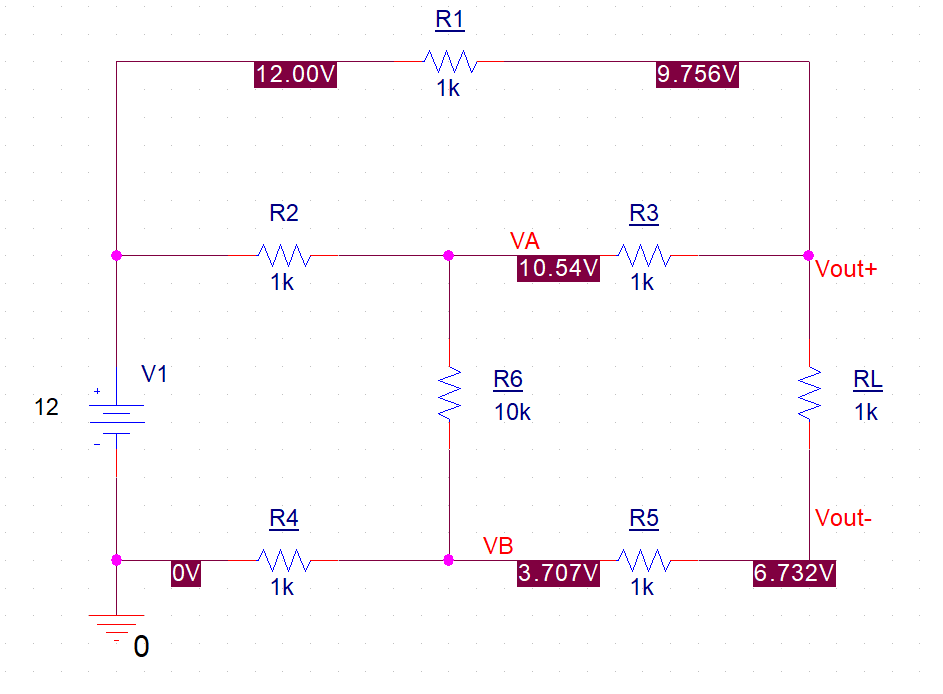
\includegraphics[height=10cm]{schematic}
	\caption{PSPICE simulation with voltage markers.}
	\label{fig:simulation}
\end{figure}

\begin{itemize}
	\item A figure of the circuit schematic should be included here.  \textbf{The ideal figure is a PSPICE image without voltage or current markers.}
	\item Define the ground in the circuit and specific nodes. \textbf{This can ideally be done by using the node labels in PSPICE.}
	\item This description can be short (about 1 paragraph in length).
\end{itemize}
\subsection{Theory: Nodal or Mesh Analysis (hand calculations)}
In this section, you should integrate the hand calculations into the text of the report.  You are required to perform either nodal or mesh analysis calculations. 
\begin{itemize}
	\item To simplify your work, you may include a scan of your hand calculations.  Be sure to number all of the equations on the right side.
	\item Show the following steps to justify the calculations:
		 \begin{itemize}
		 	\item The starting (unsimplified) simultaneous Nodal or Mesh equations
		 	\item The matrix equation used for a solution (preferably along with the simplified equation).
		 	\item The solution matrix 
		 	\item The solution of $V_{out-}$ and $V_{out}$.
		 \end{itemize}
	\item In a second paragraph, define the meaning of a \textbf{differential voltage} and calculate the theoretical value of $V_{out}$
\end{itemize}
%\subsection{Theory: Mesh Analysis (hand calculations)}
%In this section, you should integrate the hand calculations into the text of the report.  
%\begin{itemize}
%	\item Be sure to \textbf{type} the calculation, and number all equations in the body.
%	\item Show the following steps to justify the calculations:
%	\begin{itemize}
%		\item The starting (unsimplified) simultaneous Mesh equations
%		\item The matrix equation used for a solution (preferably along with the simplified equation).
%		\item The solution matrix 
%		\item The solution of all node voltages and  $V_{out}$.
%	\end{itemize}
%\end{itemize}

\subsection{Theory: PSPICE Simulation Summary}
Begin by providing a 1 paragraph description of the PSPICE setup. Was a DC simulation used, transient simulation, etc.?  Which \textbf{libraries} and \textbf{PSPICE elements} were used in the simulation? You can borrow/reuse from the text of your first tech memo here.  If you do so, please be sure to cite the tech memo.
Note that to determine the libraries used, you can find the information when you look at the properties of each element.  There will be a reference to a ``.olb'' file.  This is the library name. \textbf{As you will be likely using the same PSPICE setup throughout the term, once it is established, you may reuse the information with the permission of your instructor/TA. Cite your first lab report as a reference. In subsequent reports, you may be appending to this.} %Also, please be sure to detail the settings you have used for your Monte Carlo simulation (number of iterations, the signal selected-MAX, random number seed) so that others can recreate your work.
 
\subsubsection{PSPICE: DC Simulation }

%In this section: 
%\begin{itemize}
%	\item Refer to the screen capture of the DC Bias point simulation.  If your initial circuit schematic figure from Section \ref{Section:CircuitTopology} contains voltage makers, you do not need to include it a second time.  
%		\item Briefly comment about the results and whether they agree with your hand calculations. This should be a few sentences long
%\end{itemize}

In Figure \ref{fig:simulation} the circuit shows the results of the PSPICE simulation and all of the nodal voltages. The nodal voltage at $V_A$ and $V_B$ were $10.54\,\si\volt$ and $3.707\,\si\volt$ respectively.  

%\subsubsection{PSPICE: DC Monte Carlo Simulation }
%
%In this section, include: 
%\begin{itemize}
%	\item A figure illustrating the Monte Carlo histogram extraction of the differential voltage ($V_{out}$) and the PDF.
%	\item  Briefly comment about the results and whether they agree with your hand calculations in the context of variations to the resistors.
%\end{itemize}


\section{Hardware Experiment: Results and Discussion}
This section of the report should present what was done in hardware.  A reader should be able to recreate an experiment from the detail present.  One section discusses the equipment used in the experiment. The remaining sections discuss the results for each circuit.
\subsection{Equipment Used in the Laboratory}
Write a short paragraph to detail the equipment used in the laboratory, and specific model numbers. Ideally, you should create a table of the equipment which should be referred to in text (See Table \ref{Table:Equipment} as an example).  The room location where the experiment was performed should be included.  Note that this should be a part of all Tech Memos, as it is an essential piece for other users to replicate your experiment.  \textbf{As you will be likely using the same equipment throughout the term, once the text/tables are established, you may reuse the information with the permission of your instructor/TA. Again, cite your first lab report as a reference.}
		
		\begin{table}[h!]
			\centering
			\caption{Equipment/Software required for Lab 2.}
			\label{Table:Equipment}
			%\begin{tabular}{llllll}
				\begin{tabular}{|c||c|c|c|c|}
					\hline
					Item & Tool & Room      \\
					\hline
					Simulation & OrCAD Capture CIS & All Open EE Labs   \\	 
					\hline 
					DC Power Supply&  Agilent E3630A  & 09-3170   \\	
					\hline  
					DC Power Supply & Agilent E3631A   & 09-3200 \\ 
					\hline 
					Multimeter & Agilent 34401A & 09-3170, 09-3200 \\
					\hline
					%				Oscilloscope & Textronix TDS2012C & 09-3200  \\
					%				\hline
					%				Oscilloscope & Agilent DSO 33120A & 09-3170  \\
					%				\hline
					%				
				\end{tabular}
		\end{table}
\clearpage
\subsection{Hardware Results/Discussion}	
  Begin the section by including the experimental values of the resistors as illustrated in Table \ref{Table:Lab2Resistors}. Introduce the table in the text and briefly discuss the variation in resistance. Note that the nominal values are the ones provided in the lab handout and used in PSPICE.   
  	\begin{table}[h!]
  		\centering
  		\caption{Resistor Table}
  		\label{Table:Lab2Resistors}
  		%\begin{tabular}{llllll}
  		\begin{tabular}{|c||c|c|c|c|}
  			\hline
  			Resistor & Nominal Value (\si{\kilo\ohm})& Measured Value (\si{\kilo\ohm}) & Tolerance (\si{\percent})   \\
  			\hline
  			$R_1$ & 1 & 0.983 & 5  \\	 \hline 
  			$R_2$ & 1 & 0.983 & 5 \\	 \hline 
  			$R_3$ & 1 & 0.987 & 5 \\	 \hline 
  			$R_4$ & 1 & 0.981 & 5 \\	 \hline 
  			$R_5$ & 1 & 0.982 & 5 \\	 \hline 
  			$R_6$ & 10 & 9.95 & 5 \\	 \hline
  			$R_L$ & 1 &  0.986 & 5 \\	 \hline 
  		\end{tabular}
  	\end{table}

  	
\subsection{Hardware Results Summary}
The lab handout calls for the measuring equivalent resistance between two points in the circuits to verify the wiring.  Report the values that were obtained experimentally.  Next, include the following table per the lab documentation. Briefly summarize it. Include a discussion of the \textbf{percent error} between theory and experiment.  
	\begin{table}[h!]
		\centering
		\caption{Summary of nodal voltages for Lab 2.}
		\label{Table:Lab2DCVoltages}
		%\begin{tabular}{llllll}
		\begin{tabular}{|c||c|c|c|c|}
			\hline
			Voltage & Prelab (\si{\volt}) &  PSPICE (\si{\volt})& Hardware (\si{\volt}) & Percent Error With Hand Calc. (\si{\percent})   \\
			\hline
			$V_A$ & & 10.54 & 10.54 &\\	 \hline 
			$V_B$ & & 3.707 & 3.697 & \\	 \hline 
			$V_{out+}$ & & 9.756 & 9.764 &  \\	 \hline
			$V_{out-}$ & & 6.732 & 6.723 & \\	 \hline 
			$\Delta V_{out}=V_{out+}-V_{out-}$ &  & 3.024 & 3.040 &  \\	 \hline
		\end{tabular}
	\end{table}
	
	\section{Conclusion}
	Provide a 1 paragraph summary of the laboratory experiment.  What were the major conclusions for each part of the experiment?  Also did the theory agree with the experiment?  The conclusion is a revised version of the abstract.
	
	\section{Acknowledgments}
	Acknowledge \textbf{any} source of help received in the experiment/writing the report.  This should certainly include your lab partner/teaching assistant/instructor.  It may also include other classmates/study partners. State briefly what the nature of the help was.
	
	\textbf{Your report should include references to appropriate pages in the text, as well as any other sources, websites/etc. consulted in the preparation of the report.}
\begin{thebibliography}{9}
	\bibitem{AlexanderSadiku}
	C.K. Alexander, and M.K.O. Sadiku,
	\emph{Fundamentals of Electric Circuits, 4th Edition},
	McGraw Hill, pp. xx-yy(EDIT), 2009.
	\bibitem{OldLab}
A. Student,
	\emph{EEEE 281 Lab 1 Tech Memo},
	page xx-yy, submitted Month, Day, 2015.
	\bibitem{RommelLab}
	S. Rommel,
	\emph{EEEE 281 Lab 1 Lecture notes},
	slides xx-yy, Spring 2015.
\end{thebibliography}

\end{document}



